\section{Metodologi}

% Slide 12: Bab 3.1 - Alur Penelitian
\begin{frame}{Bab 3.1 - Alur Penelitian}
    \centering
    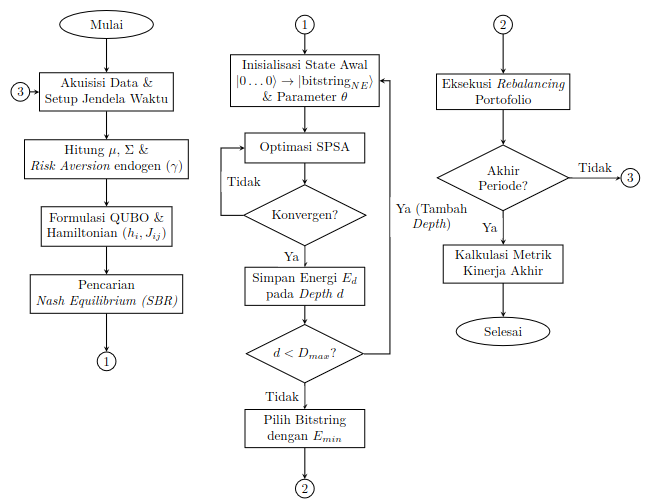
\includegraphics[width=0.6\textwidth]{Gambar/31_Dialir.png}
\end{frame}

% Slide 13: Bab 3.2 - Akuisisi dan Pra-pemrosesan Data
\begin{frame}[fragile]{Bab 3.2 - Akuisisi dan Pra-pemrosesan Data}
    \begin{algorithm}[H]
        \footnotesize
        \begin{algorithmic}[1]
            \Procedure{DataPreprocessing}{tickers, $t_{start}, t_{end}$}
                \State $\mathbf{P} \gets \text{DownloadClosingPrice}(tickers)$
                \State $r_{log} \gets \ln(\mathbf{P}_{t} / \mathbf{P}_{t-1})$ \Comment{Kalkulasi \textit{Log Return}}
                \State $\mu_{log} \gets \text{Mean}(r_{log}) - 0.5 \cdot \text{Var}(r_{log})$ \Comment{\textit{Volatility Drag}}
                \State $\Sigma \gets \text{Covariance}(r_{log})$
                \State $\gamma \gets \text{ComputeEndogenousLambda}(\mu_{log}, \Sigma)$
                \State \Return $\mu_{log}, \Sigma, \gamma$
            \EndProcedure
        \end{algorithmic}
    \end{algorithm}
\end{frame}

% Slide 14: Bab 3.3 - Pemodelan Hamiltonian Portofolio
\begin{frame}[fragile]{Bab 3.3 - Pemodelan Hamiltonian Portofolio}
    \begin{algorithm}[H]
        \footnotesize
        \begin{algorithmic}[1]
            \Procedure{BuildHamiltonian}{$\mu, \Sigma, \gamma, K, \lambda$}
                \State $Q_{ii} \gets \frac{\gamma \Sigma_{ii}}{2K^2} - \frac{\mu_i}{K} + \lambda(1 - 2K)$
                \State $Q_{ij} \gets \frac{\gamma \Sigma_{ij}}{2K^2} + \lambda$
                \State $h_i \gets -\frac{1}{2} (Q_{ii} + \sum_{j \neq i} Q_{ij}), \quad J_{ij} \gets \frac{1}{4} Q_{ij}$
                \State $H \gets \sum h_i \hat{Z}_i + \sum J_{ij} \hat{Z}_i \hat{Z}_j + C \cdot I$
                \State \Return $H$
            \EndProcedure
        \end{algorithmic}
    \end{algorithm}
\end{frame}

% Slide 15: Bab 3.4 - Algoritma Nash Sequential Best Response
\begin{frame}[fragile]{Bab 3.4 - Algoritma Nash Sequential Best Response}
    \begin{algorithm}[H]
        \scriptsize
        \begin{algorithmic}[1]
            \Procedure{NashSBR}{$\mu, \Sigma, \gamma, N, K$}
                \State $x \gets \text{InitialSelection}(K)$
                \For{$iter = 1$ to $max\_iter$}
                    \For{$i \in S_{in}$ and $j \in S_{out}$}
                        \State $x' \gets \text{Swap}(x, i, j)$
                        \If{$\Phi(x') > \Phi(x)$}
                            \State $x \gets x', \Phi \gets \Phi', improved \gets \text{True}$
                            \State \textbf{break}
                        \EndIf
                    \EndFor
                    \If{not $improved$} \textbf{break} \EndIf
                \EndFor
                \State \Return $x$ \Comment{Warm-start Bitstring}
            \EndProcedure
        \end{algorithmic}
    \end{algorithm}
\end{frame}

% Slide 16: Bab 3.5 - Optimasi Variasional HE-VQE Adaptif
\begin{frame}[fragile]{Bab 3.5 - Optimasi Variasional HE-VQE Adaptif}
    \begin{algorithm}[H]
        \scriptsize
        \begin{algorithmic}[1]
            \Procedure{AdaptiveVQE}{$H, x_{NE}, D_{max}, \lambda_{target}$}
                \State $\theta \gets \text{InitialParameters}(x_{NE})$
                \For{$d = 1$ to $D_{max}$}
                    \For{$k = 1$ to $N_{iter}$}
                        \State $\lambda_k \gets \text{PenaltyAnnealing}(k)$
                        \State $\mathcal{L}(\theta) \gets \langle \psi(\theta) | H_{obj} + \lambda_k H_{pen} | \psi(\theta) \rangle$
                        \State $\theta \gets \theta - a_k \cdot \text{SPSA\_Gradient}(\mathcal{L}, \theta)$
                    \EndFor
                    \State $\theta \gets \text{LayerExpansion}(\theta)$
                    \If{$\text{Converged}(\theta)$} \textbf{break} \EndIf
                \EndFor
                \State \Return $x^* \gets \text{Argmax}(|\langle x | \psi(\theta_{final}) \rangle|^2)$
            \EndProcedure
        \end{algorithmic}
    \end{algorithm}
\end{frame}

% Slide 17: Bab 3.6 - Simulasi Backtesting dan Metrik Evaluasi
\begin{frame}[fragile]{Bab 3.6 - Simulasi Backtesting dan Metrik Evaluasi}
    \begin{algorithm}[H]
        \scriptsize
        \begin{algorithmic}[1]
            \Procedure{BacktestLoop}{$Data, K$}
                \For{$t \in \text{Timeline}$}
                    \State $\mu, \Sigma, \gamma \gets \text{DataPreprocessing}(Data_{train})$
                    \State $H \gets \text{BuildHamiltonian}(\mu, \Sigma, \gamma, K)$
                    \State $x_{NE} \gets \text{NashSBR}(\mu, \Sigma, \gamma, K)$
                    \State $x^*_t \gets \text{AdaptiveVQE}(H, x_{NE})$
                    \State $R_t \gets \text{ExecuteRebalance}(x^*_t)$
                \EndFor
                \State \Return $\text{PerformanceMetrics}$
            \EndProcedure
        \end{algorithmic}
    \end{algorithm}
\end{frame}

% Slide 18: Bab 3.7 - Validasi Solusi Eksak Brute Force
\begin{frame}[fragile]{Bab 3.7 - Validasi Solusi Eksak Brute Force}
    \begin{algorithm}[H]
        \footnotesize
        \begin{algorithmic}[1]
            \Procedure{BruteForceValidation}{$H, N, K$}
                \State $best\_energy \gets \infty$
                \For{each $x \in \text{Combinations}(N, K)$}
                    \State $E \gets \text{CalculateIsingEnergy}(x, H)$
                    \If{$E < best\_energy$}
                        \State $best\_energy \gets E, best\_x \gets x$
                    \EndIf
                \EndFor
                \State \Return $best\_x, best\_energy$
            \EndProcedure
        \end{algorithmic}
    \end{algorithm}
\end{frame}
